\section{interaction quench}

\begin{figure}[H]
%\centering
\begin{subfigure}{.5\textwidth}
 % \centering
 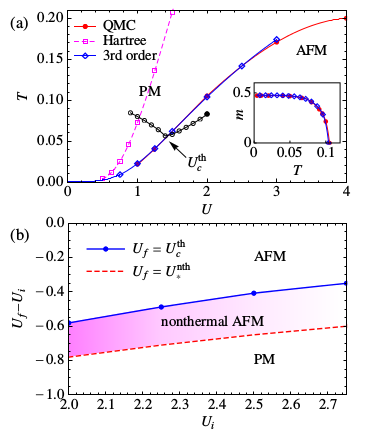
\includegraphics[width=0.9\linewidth]{interaction_quench_AFM/AFM_DMFT_phase.png}
  \caption{HF}
  %\label{fig:sub1}
\end{subfigure}%
\begin{subfigure}{.5\textwidth}
 % \centering
  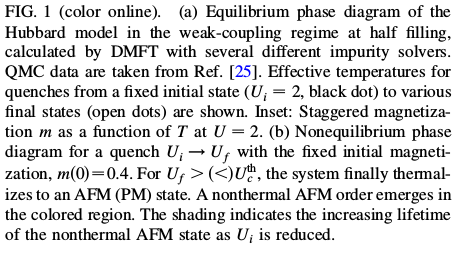
\includegraphics[width=0.9\linewidth]{interaction_quench_AFM/AFM_DMFT_phase_text.png}
  \caption{DMFT}
  %\label{fig:sub2}
\end{subfigure}
%\caption{dos for $\Delta=1.0t$, $t_2 = 0.4t$(a) at U = 0.4t band insulator  (b) at U = 2.0t metal}
%\label{fig:test}
\end{figure}


\begin{figure}[H]
%\centering
\begin{subfigure}{.5\textwidth}
 % \centering
 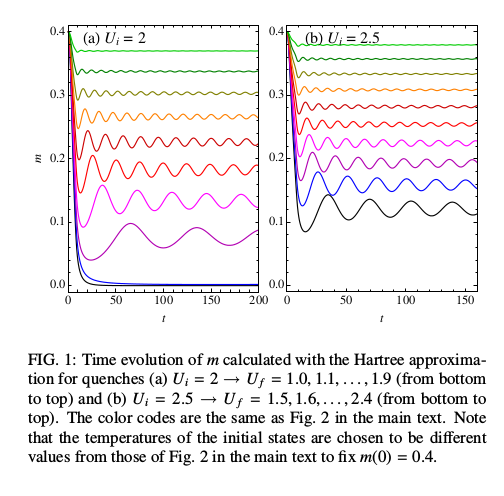
\includegraphics[width=0.9\linewidth]{interaction_quench_AFM/AFM_HF_m.png}
  \caption{HF}
  %\label{fig:sub1}
\end{subfigure}%
\begin{subfigure}{.5\textwidth}
 % \centering
  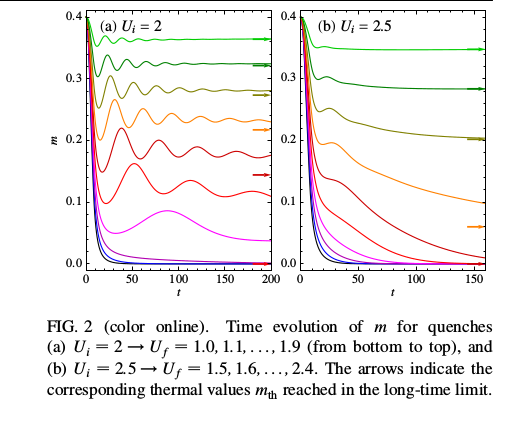
\includegraphics[width=0.9\linewidth]{interaction_quench_AFM/AFM_DMFT_m.png}
  \caption{DMFT}
  %\label{fig:sub2}
\end{subfigure}
%\caption{dos for $\Delta=1.0t$, $t_2 = 0.4t$(a) at U = 0.4t band insulator  (b) at U = 2.0t metal}
%\label{fig:test}
\end{figure}


%\begin{figure}[H]
%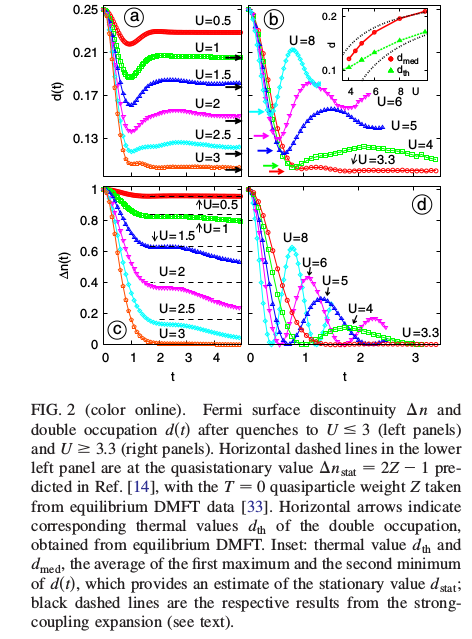
\includegraphics[width=0.8\linewidth]{interaction_quench/Hubbard_model.png}
%  \caption{\cite{HUB_para}}
%\end{figure}

for the Hubbard model we see that steady double occupancy is larger than the equilibrium value. where as for IHM case its is lower 
